\documentclass[12pt,a4paper]{article}

\usepackage{float}
\restylefloat{figure}
\usepackage{hyperref}
\usepackage{graphicx}
\usepackage{gensymb}
\usepackage[title]{appendix}
\usepackage[dotinlabels]{titletoc}
\usepackage[nottoc,numbib]{tocbibind}
\usepackage{mathtools}
\usepackage[margin=0.5in]{geometry}
\renewcommand{\thefootnote}{\arabic{footnote}}

\newcommand*\wrapletters[1]{\wr@pletters#1\@nil}
\def\wr@pletters#1#2\@nil{#1\allowbreak\if&#2&\else\wr@pletters#2\@nil\fi}

\usepackage{enumitem}
\setenumerate{itemsep=0pt}

% Add support for multi-page tables.
\usepackage{longtable}

\pagenumbering{arabic}

\title{EE4DNA Coursework 4}
\author{Chris Cummins}

\begin{document}
\maketitle

\section{Implementing Items}

Actions on items are implemented by the
\texttt{adventure.actions.Take} and \texttt{adventure.actions.Release}
classes, and stored as a HashSet in \texttt{adventure.RoomImpl} whose
contents are modified during the \texttt{player\_entered()} and
\texttt{player\_left()} callbacks. Access to the HashSet is
synchronized so as to prevent concurrency issues that would arise from
multiple players simultaneously performing actions on the same item.

\section{Managing Access to a Shared Resource}

Mutually exclusive access to a shared resource is demonstrated in the
\texttt{adventure.actions.GuessTheNumber} class, which implements a
trivial game of guess the number, with the one precondition that only
a single player may play at a time. In order to achieve this, the
current player's user name is used as a locking mechanism, with the
lock being acquired when the player beings the game, and freed when
the player completes the game. Additionally, the lock is freed if the
player leaves the room, preventing the scenario of a player leaving
the game or changing room and preventing other users from accessing
the game resource. A scenario was arranged to test this edge case with
two players:

\begin{figure}[H]
  \centering
  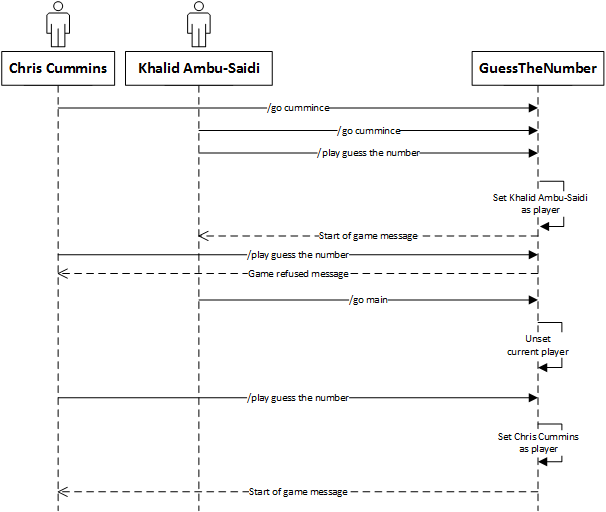
\includegraphics[width=5.5in]{assets/sequence.png}
\end{figure}

The server log shows the sequence of events:

\begin{verbatim}
Mon Mar 17 20:29:40 GMT 2014 OK:      player_entered(cummince:Christopher Cummins)
Mon Mar 17 20:30:33 GMT 2014 OK:      player_entered(ambuskas:Khalid Ambu-Saidi)
Mon Mar 17 20:31:16 GMT 2014 OK:      gtn: Player ambuskas started game
Mon Mar 17 20:31:35 GMT 2014 OK:      gtn: Locked cummince from existing game
Mon Mar 17 20:31:44 GMT 2014 OK:      gtn: Player ambuskas left room
Mon Mar 17 20:31:44 GMT 2014 OK:      player_left(ambuskas:Khalid Ambu-Saidi)
Mon Mar 17 20:31:57 GMT 2014 OK:      gtn: Player cummince started game
\end{verbatim}

And the relevant commands from my client session:

\begin{verbatim}
> /play guess the number
[20:31:35] Khalid Ambu-Saidi is already playing!
[20:31:44] Khalid Ambu-Saidi has left the room.
> /play guess the number
[20:31:57] Welcome to guess the number! Type /guess followed by your first guess
\end{verbatim}


\section{Persistent State}

An example of persistent state is included in the
\texttt{adventure.actions.Message} class, which implements the read
and write actions for persistent messages. Messages are written and
read in a line by line fashion to a per-room messages file:

\begin{verbatim}
"Hello, everyone!" - Christopher Cummins
"This is a message to you Rudy" - Christopher Cummins
\end{verbatim}

\end{document}
